\documentclass[twoside,f1]{HsH-report}

\usepackage{color}
\usepackage{lipsum}
\usepackage{siunitx}
\usepackage{biblatex}
\usepackage{soul}
\addbibresource{bib/localBibliography.bib}

\begin{document}

\pagenumbering{Roman}
\maketitle
\declarationAuthorship

\begin{abstract}
	\lipsum[5-8]
\end{abstract}

\tableofcontents

\cleardoublepage % unbedingt erforderlich bei Doppelseitigem layout vor neuer Seitennummerierung!
\pagenumbering{arabic} % Seitennummerierung normale zahlen

\chapter{one}
	\label{chap: one}
	{\color{red}test} und stuff
	\begin{figure}
		\centering
		
\includegraphics[width=.6\textwidth]{img/lorem-ipsum.jpg}
		\caption{test}
	\end{figure}

	noch ein test \normalsubscripts$R_t$ \upsubscripts$R_t$

	mit einheit: $R=200\,\milli\ohm+ \SI{0.34567453}{\volt\per\metre}$
	\cite{laboranleitung:physik}
	\vspace{2cm}\\
	eine zahl: $3,5+3.5$\footnote[1]{hello}\\

	Tiny: {\tiny hello} Small: {\small hello}

	\makeatletter
	\newcommand{\test}[1][l]{
		{
			\def\t{#1}
			\if\t l left
			\else
				right
			\fi
		}
	}
	\test; \test[right]

	\lipsum[5-6]

	\pagebreak
	\begin{figure}
		\centering
		\includegraphics[width=0.6\textwidth, page=2]{plt/build/examplePlot.pdf}
		\caption{a nice plot}
	\end{figure}

	\begin{figure}
		\centering
		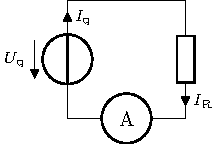
\includegraphics{crc/build/exampleCircuit.pdf}
		\caption{a circuit diagramm}
	\end{figure}

	\makeatletter

	\begin{figure}
		\graphicspath{{svg/build/}} % double curly brackets needet for unknown reason
		\input{svg/build/exampleSVG.pdf_tex}
		\caption{made via inkscape}
	\end{figure}

	\begin{table}
		\caption{hello}
		\begin{tabular}{c|c}
			test & hello \\\hline\hline
			1 & 2 \\
			\multicolumn{2}{|c|}{temp}
		\end{tabular}
	\end{table}

\printbibliography
\listoffigures
\end{document}
